\chapter{Grafos}
\label{cap:grafos}

Grafos são estruturas discretas que consistem em vértices, e arestas que
conectam estes vértices. Existem vários tipos de grafos, dependendo da
existência de uma direcção nas arestas, de acordo a possibilidade de várias
arestas se interligarem ao mesmo par de vértices e de acordo a existência de
\emph{loops} ou repetições.
Problemas em quase todas as disciplinas podem resolvidos utilizando modelos de
grafos. Iremos apresentar alguns exemplos para ilustrar como os grafos são
utilizados como modelos numa variedade de aéras. Por exempo, iremos mostrar como
os grafos são utilizados para representar a competição de diferentes espécias
num nicho ecológico, e como os grafos são usados para representar quem
influencia quem numa organização e etc.

Utilizando modelos de grafos, podemos determinar se é possível caminhar todas as
ruas de uma cidade sem psasar por uma rua duas vezes, e podemos determinar o
número de cores necessário para colorar as regiões de um mapa. Grafos podem ser
utilizados para determinar se um circuito pode ser implementado numa placa de
circuitos plana. Podemos distinguir entre dois compostos químicos com a mesma
fórmula molecular mas estruturas diferentes utilizando grafos. Podemos
determinar se dois computadores estão conectados por um \emph{link} de
comunicação utilizando modelos gráficos de redes. Grafos com pesos atribuidos as
suas arestas podem ser utilizados para resolver problemas como encontrar o
caminho mais curto entre duas cidades numa rede de transporte. Neste capítulo
iremos apresentar os conceitos básicos da teoria dos grafos e apresentar alguns
modelos de grafos. Para resolver uma boa parte dos problemas que podem ser
estudados utilizando grafos, iremos apresentar alguns algoritmos de grafos.
Iremos também estudar a complexidade destes algoritmos.

\section{Grafos e Modelos de Grafos}

Começamos com a definição de grafos.
\begin{defn}
\label{def51}
Um \emph{grafo} $G = (V,E)$ consiste em $V$, um conjunto não-vazio de
\emph{vértices} (ou \emph{nós}) e $E$, um conjunto de \emph{arestas}. Cada
aresta possui ou um ou mais vértices associados a esta, chamada de sua
\emph{extremidade}. Diz-se que uma aresta \emph{conecta} as suas extremidades.
\end{defn}

\begin{description}
\item[\emph{Nota}:] O conjunto de vértices $V$ de um grafo $G$ pode ser
infinito. Um grago com um conjuntos infinito de vértices ou um
número infinito de arestas é chamado de \textbf{grafo infinito}, e em comparação, um grafo com
um conjunto de finito de vértices e um conjunto finito de arestas é chamado de
\textbf{grafo finito}. Neste manual iremos considerar apenas grafos finitos.
\end{description}

Agora imagine que uma rede de computadores é formada por centros de dados e
\textit{links} de comunicação entre computadores. Podemos representar a
localização de cada centro de dados por um ponto e cada \textit{link} de
comunicação por um segmento de linha, como mostra a Figura \ref{fig51}

\begin{figure}[H]
	\centering
	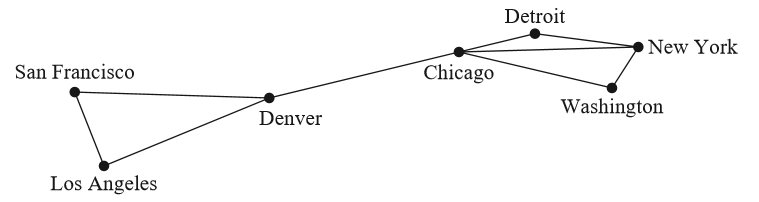
\includegraphics[scale=1]{chapter/imagens/51}
	\caption{Uma Rede de Computadores.}
	\label{fig51}
\end{figure}

Esta rede de computadores pode ser modelada utilzando grafos em que os vértices
do grafo representam centros de dados e as areas representam os \textit{links}
de comunicação. No geral, visualizamos os grafos usando pontos para represtentar
os vértices e segmentos de linha, possivelmente curvos, para representar as
arestas, onde as extremidades de um segmento de linha representando uma aresta
são os pontos representando as extremidades da aresta. Quando desenhamos um
grafo, geralmente tentamos desenhar as arestas de formas a não se cruzarem. No
entanto, isto não é necessário porque qualquer representação utilizando pontos
para representar os vértices e qualquer forma de conexão entre os vértices pode
ser utilizada. De facto, existem alguns grafos que não podem ser desenhados no
plano sem que as arestas se cruzem (veja a Secção \ref{sec:107}). O ponto
principal é que a forma como desenhamos um grafo é arbritária, desde que as
conexões correctas entre os vértices estejam representadas.

Note que cada aresta do grafo representando esta rede de computadores conecta
dois vértices diferentes. Isto é, nenhuma aresta conecta um vértice a si
próprio. Além disso, duas arestas diferentes não conectam o mesmo par de
vértices. Um grafo em que cada aresta conecta dois vértices diferentes e em que
duas arestas conectam o mesmo par de vértices é chamada de \textbf{grafo
simples}. Note que num grafo simples, cada aresta está associada à um par
não-ordenado de vértices, e mais nenhuma aresta está associada a esta mesma
aresta. Consequentemente, quando existe uma aresta de um grafo simples associada
a $\{u,v\}$, também podemos dizer, sem possibilidade de confusão, que $\{u,v\}$
é uma aresta do grafo.

Uma rede de computadores pode conter múltiplas ligações entre centros de dados,
como ilustrado na Figura \ref{fig52}. Para modelar tais redes precisamos de
grafos que posuam mais de uma aresta conectando o mesmo par de vértices. Grafos
que possam ter \textbf{múltiplas arestas} a conectar os mesmos vértices são
chamados de \textbf{multigrafos}. Quando existem $m$ arestas diferentes
associadas ao mesmo par não-ordenado de vértices $\{u,v\}$, também dizemos que
$\{u,v\}$ é uma aresta de multiplicidade $m$. Isto é, podemos pensar neste
conjunto de arestas como $m$ diferentes cópias de uma aresta $\{u,v\}$.

\begin{figure}[H]
	\centering
	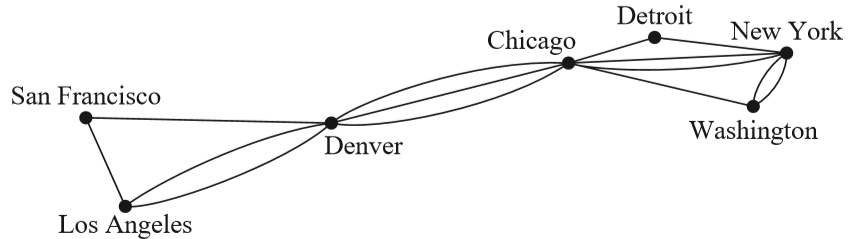
\includegraphics[scale=1]{chapter/imagens/52}
	\caption{Uma Rede de Computadores com Múltiplos LInks entre Centros de Dados.}
	\label{fig52}
\end{figure}

Por vezes um \textit{link} de comunicação de conecta um centro de dados consigo
próprio, possivelmente um laço de realimentação para diagnóstico. Uma rede deste
tipo é ilustrada na Figura \ref{fig53}. Para modelar esta rede precisamos
incluir arestas que conectem um vértice consigo próprio. Tais arestas são
chamadas de \textbf{laços} e as vezes

\begin{figure}[H]
	\centering
	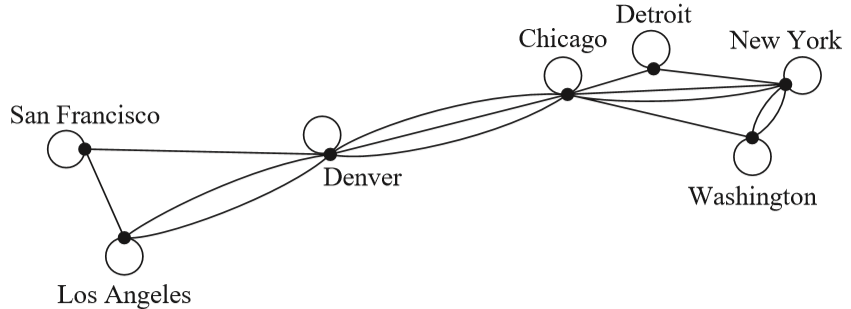
\includegraphics[scale=1]{chapter/imagens/53}
	\caption{Uma Rede de Computadores com Links para Diagnósticos.}
	\label{fig53}
\end{figure}


